
\documentclass{acm_proc_article-sp}

%!TEX root = ./Milestone1.tex

% !TEX root =  ./VersionPaper.tex
\usepackage[english]{babel}
\usepackage{threeparttable}
\usepackage{amssymb}
\setcounter{tocdepth}{3}
\usepackage{graphicx}
\usepackage{multirow}
\usepackage{url}
\usepackage{array}
\usepackage{xspace}
\usepackage{moreverb}
\usepackage{listings}
\usepackage{color}
\usepackage{cite}
\usepackage{relsize}
\usepackage{color}
%\usepackage{wasysym}
\usepackage{fancybox}
\usepackage{balance}
\usepackage{enumitem}
\usepackage{lmodern}
\usepackage[style=base]{caption}
\usepackage{subcaption}
\usepackage{epstopdf}

\usepackage{amsmath}

\newcommand{\version}[1]{\normalsize{Version #1 - \mydate\today\xspace,\xspace\currenttime}}

%\newdateformat{mydate}{\monthname[\THEMONTH]\xspace\THEDAY}

\newcommand{\fixme}[1]{\textcolor{red}{#1}}
\newcommand{\TODO}[1]{\textcolor{magenta}{\textbf{TODO: }#1}}
\newcommand{\feedback}[1]{\textcolor{magenta}{\textbf{ASK: }#1}}


\newcommand{\figchoice}[1]{\fontfamily{pcr}\selectfont \textit{#1}}
\newcommand{\figvn}[1]{\fontfamily{pcr}\selectfont  \textbf{#1}}

\newcommand{\ADD}[1]{\textbf{\textcolor{blue}{#1}}}
\newcommand{\REMOVE}[1]{\textbf{\textcolor{red}{#1}}}



\newcommand{\mybox}[1]{
\begin{center}
\setlength{\fboxsep}{5pt}%
\Ovalbox{%
\begin{minipage}{.45\textwidth}
\begin{center}
{\it #1} 
\end{center}
\end{minipage}}
\end{center}
}

\lstdefinelanguage{CSharp}
{
sensitive=true,
morekeywords=[1]{
abstract, as, async, await, base, break, case,
catch, checked, class, const, continue,
default, delegate, do, else, enum,
event, explicit, extern, false,
finally, fixed, for, foreach, goto, if,
implicit, in, interface, internal, is,
lock, namespace, new, null, operator,
out, override, params, private,
protected, public, readonly, ref,
return, sealed, sizeof, stackalloc,
static, struct, switch, this, throw,
true, try, typeof, unchecked, unsafe,
using, virtual, volatile, while, bool,
byte, char, decimal, double, float,
int, lock, object, sbyte, short, string,
uint, ulong, ushort, void},
morecomment=[l]{//},
morecomment=[s]{/*}{*/},
morecomment=[l][keywordstyle4]{\#},
morestring=[b]",
morestring=[b]',
}

\lstset{ %
%frame=bottom,
  language=CSharp,                % the language of the code
  basicstyle=\ttfamily\scriptsize,           % the size of the fonts that are used for the code
  keywordstyle=\color{blue},
  commentstyle=\color{mygreen},
  numberstyle=\tiny\color{mygray}
  stringstyle=\color{mymauve},
  rulecolor=\color{black}, 
  stepnumber=1,                   % the step between two line-numbers. If it's 1, each line 
  %numbers=left,                   % where to put the line-numbers
  numberstyle=\scriptsize,  
  numbersep=5pt,  
  showspaces=false,               % show spaces adding particular underscores
  showstringspaces=false,         % underline spaces within strings
  showtabs=false,                 % show tabs within strings adding particular underscores
  tabsize=2,                      % sets default tabsize to 2 spaces
  breaklines=false,                % sets automatic line breaking
  breakatwhitespace=false,        % sets if automatic breaks should only happen at whitespace
  belowskip=1pt,
  aboveskip=2pt
}


\newcommand{\codesnippet}[1]{
\begin{lstlisting}#1\end{lstlisting}}

\newcommand{\readme}[1]{#1}

\newcommand{\etal}{\emph{et~al}.~}
\newcommand{\Comment}[1]{}%\textbf{\textsl{$\langle\!\langle$#1$\rangle\!\rangle$}}}
\newcommand{\spacedinlineheader}[1]{\vspace{1.5 mm} \noindent \textbf{#1}}
\newcommand{\Space}[1]{}

\newcommand{\website}{http our web site\xspace}
\newcommand{\TotalNumProjects}{59\xspace}
\newcommand{\TotalVNs}{8686\xspace}
\newcommand{\numberchoices}{\textit{number of choices for assigning a new version number}\xspace}
\newcommand{\numberichoices}{\textit{number of immediate choices for assigning a new version number}\xspace}
\newcommand{\numberextrachoices}{\textit{number of additional choices for assigning a new version number}\xspace}
\newcommand{\choices}{\textit{choices for assigning a new version number}\xspace}
\newcommand{\choice}{\textit{choice for assigning a new version number}\xspace}

\newcommand{\code}[1]{\begin{small}\texttt{#1}\end{small}}
\newcommand{\URL}[1]{\begin{footnotesize}\url{#1}\end{footnotesize}}

\newcommand{\Analyzer}{\begin{small}\textsc{VersionAnalyzer}\end{small}\xspace}

\newcommand{\subParagraph}[1]{\textbf{\emph{#1}}}
\newcommand{\MyParagraph}[1]{\noindent \textbf{#1}}

% % % % Paper specific Commands % % % % %

\newcommand{\mysubitem}[1]{\begin{itemize}\item[] #1 \end{itemize}}

\newcommand{\mac}{\textsuperscript{$\star$\space}}
\newcommand{\windows}{\textsuperscript{$\Box$\space}}
\newcommand{\ios}{\textsuperscript{$\bullet$\space}}
\newcommand{\android}{\textsuperscript{$\dagger$\space}}
\newcommand{\linux}{\textsuperscript{$\Diamond$\space}}

\newcommand{\NumTotalApps}{36\space}
\newcommand{\NumMobileApps}{12\space}
\newcommand{\NumDesktopApps}{12\space}
\newcommand{\NumSiblingpApps}{12\space}

\newcommand{\MinNumReleases}{3\space}
\newcommand{\TotalNumReleases}{288\space}

\newcommand{\RQOne}{\textbf{RQ1:} Do mobile applications exhibit more frequent releases than desktop applications?}
\newcommand{\RQTwo}{\textbf{RQ2:} Do applications with siblings behave more like mobile or desktop apps?}
\newcommand{\RQThree}{\textbf{RQ3:} Are bugs/features/enhancements more common in desktop, mobile, or sibling applications?}

\newcommand{\sibs}{sibling applications\space}
\newcommand{\sib}{sibling application\space}

\newcommand{\eg}{e.g.,\space}
\begin{document}

\title{What's in a release platform? }

\numberofauthors{2} 
\author{
\alignauthor
Kendall Bailey \\
       \affaddr{Oregon State University}
% 2nd. author
\alignauthor
Hongyan Yi \\
       \affaddr{Oregon State University}
}

\maketitle
\begin{abstract}

With the recent explosion of mobile development, this paper looks at the differences between mobile and desktop applications from the perspective of release notes.
With the growth of mobile development, there has also been an emergence of applications that exist on both platforms that no one has yet tried to characterize.
This class of applications, which we call sibling applications, does not adhere to the behavior of either mobile or desktop applications, instead appearing to be a distinct group.
Sibling applications and the information about desktop and mobile applications can be used by developers to better understand where to spend time when developing.

\end{abstract}

% A category with the (minimum) three required fields
 %\category{H.4}{Information Systems Applications}{Miscellaneous}
%A category including the fourth, optional field follows...
%\category{D.2.8}{Software Engineering}{Metrics}[complexity measures, performance measures]

\section{Introduction}

It has been believed by the software community that mobile application release cycles are shorter than desktop release cycles. 
The rapid rise of mobile technology has changed expectations from consumers and added pressure to developers to take advantage of new technology and quickly push it to the market.
This fast-paced business model gels with agile and extreme programming methodologies.

Companies know that mobile applications now represent a large segment of the market and often provide both mobile and desktop versions of their software to reach the most consumers possible.
The growing group of applications that belong to both mobile and desktop applications have not yet been looked at as single distinct group.
In this paper we analyze some of the properties of these application ``siblings.''

\MyParagraph{Siblings: }We define \textbf{\sibs} as applications that have the same name and are released by the same company for different platforms. 
For this research \sibs refers to a mobile application (iOS or Android) and desktop application (OSX, Windows Vista/7/8, or Linux) pairing.
An example of \sibs would be OmniGraffle, which maintains both a iOS and OSX application of the same name with different version histories, though often version histories of sibling applications are not separated.


In this paper we collected the release notes from \NumDesktopApps desktop applications, \NumMobileApps mobile applications, and \NumSiblingpApps sibling applications. 
If we maintain our minimum number of releases at \MinNumReleases releases, this gave us \TotalNumReleases releases and \TotalNumStatements statements to use for analysis.

Our analysis focuses on the length of release cycles of the different types of applications and the contents of the releases to answer our three research questions.

\begin{itemize}
\item \RQOne
\item \RQTwo
\item \RQThree
\end{itemize}

In the course of our research we found that:
\begin{itemize}
\item Mobile application release cycles are shorter than desktop release cycles
\item In reference to release cycles, sibling applications behave like mobile applications
\item Desktop applications tend to have more bug fixes in each release
\item Sibling applications tend to have fewer features per release
\item Desktop applications tend to have more enhancements in each release
\end{itemize}


%\keywords{ACM proceedings, \LaTeX, text tagging} % NOT required for Proceedings
%\section{Experimental Setup}
\section{Procedure}
We collected the release notes or change logs of suitable applications that consist of a healthy mix of mobile applications, desktop applications, or  mobile applications with a desktop applications sibling. 
Suitable applications will have:

\begin{enumerate}
	\item A version history length of at least \MinNumReleases releases
	\item The date of each release
	\item Release notes that mention bugs, features, enhancements, etc.
\end{enumerate}

To collect the data we grab text from any release histories found on the application developers' website or application distributors' documentation. 
%To get release history data from locations that block conventional copy and pasting (\eg iTunes), we spoof the iTunes user agent to retrieve the needed documentation. \feedback{Should we admit to this?}

As the granularity of change, we chose release histories because it allowed for more similar analysis of statements in both open source and proprietary applications. 
Often, open source applications allow users to view the open and closed issues across the history of the applications. 
The bugs/features/enhancements are reported by and communicated to users with high technical skills. 
However because releases can span many commits, release notes are often more general than the notes from each commit.

Proprietary applications tend to be more vague in their descriptions of the contents of each release to prevent lost of customer confidence and to protect their intellectual property. 
Proprietary applications also appeal to a wider audience who have a collectively lower level of technological understanding which also affects the level of the language chosen.

\begin{table*}[t]
\centering
			\begin{tabular}{|c|c|c|} \hline
				\multicolumn{3}{|c|}{\large Mobile Applications}\\ \hline 
				\textbf{Afterlight\ios} & \textbf{CNN\ios} & Clash of Clans\ios \\
				\textbf{Credit Karma\ios} & Crittercisms\android & \textbf{Dictionary\ios} \\
				Evernote Food\ios & \textbf{Facebook Messenger\ios} & \textbf{Heads Up\ios}  \\
				\textbf{Instagram\android} & \textbf{Instapaper\ios} & \textbf{Luminosity\ios}  \\
				\textbf{New Words with Friends\android} & \textbf{Pandora\ios} & Plague Inc\ios \\
				\textbf{Run Keeper\ios} & \textbf{Sleep Cycle Alarm\ios} & \textbf{Songza\ios} \\
				\textbf{Wish\ios} & \textbf{Youtube\ios} & \\\hline
		\end{tabular}
\vspace{.5cm}
	
	\begin{tabular}{c c}
		\begin{tabular*}{.5\textwidth}{|c|c|}  \cline{1-2}
		
			\multicolumn{2}{|c|}{\large Desktop Applications} \\  \cline{1-2}

			Acorn\mac & Aptana\windows\mac\linux \\
			\textbf{Charles\windows\mac\linux} & GameMaker\windows \\
			\textbf{Kaleidoscope\mac} & Kerbal Space Program\windows\mac\linux \\
			NDepend\windows & \textbf{NetNewsWire\mac} \\
			Tableau\windows & VM Ware Fusion\mac \\
			Valgrind\linux & \textbf{Versions\mac} \\  \cline{1-2}
		\end{tabular*}	
	&
	\begin{tabular*}{.5\textwidth}{|c|c|} \cline{1-2}
			\multicolumn{2}{|c|}{\large Sibling Applications} \\  \cline{1-2}
			1Password\mac\ios & \textbf{Bastion\windows\mac\linux\ios} \\
			\textbf{Covenant Eyes\windows\android} & \textbf{Creative Cloud\windows\mac\ios} \\
			\textbf{Dashlane\mac\windows\ios} & OmniGraffle\mac\ios \\
			\textbf{Raptr\windows\ios} & \textbf{SplashID\mac\android} \\
			\textbf{Spotify\windows\mac\linux\android} & \\  \cline{1-2}
		\end{tabular*}	

	\end{tabular}

	\caption{Our corpus divided into the three categories: Mobile, Desktop, and Sibling applications. Bolded application names indicate we classified the release notes of those applications. The superscript symbols represent the platform from which each of the release notes was taken and are as follows: \ios indicates iOS applications, \android indicates Android applications, \windows indicates Windows applications, \mac indicates OSX applications, \linux indicates Linux applications. For desktop applicaitons, if the source of the release notes did not indicate to which platform the release notes specifically related all possible platforms are marked.}
	\label{tab:corpus}
\end{table*}

In choosing our corpus we tried to not focus on a certain genre of application while still choosing popular applications from the top sellers/downloads lists provided by distributors.
We also tried to maintain a balance of Android and iOS applications. On the occasion that an application had release notes for multiple platforms and each platform had differentiated release notes, only one platform's application was chosen to add to the corpus.
Table~\ref{tab:corpus} shows the contents of our corpus and how we classified each application.

Using the data from our corpus, we first analyzed the release cycles of the different categories of applications. This was done using each release in the corpus listed in Table~\ref{tab:corpus}. 


Then, we classified each of the statements within the release notes to fall into one of six categories: bugs, enhancements, features, non-functional requirements, gratitude, and feedback/contact.
Statements which describe two or more changes are split into atomic parts for more accurate classification.
%\TODO{Add historgram results of common word usages for each category}

\MyParagraph{Bugs: }The bugs category describes statements in release notes that correct flaws within the application.
An example of a statement belonging in the bugs category is "Fixed a crash when closing documents while there was an active text insertion point."
%Statements belonging to the bugs category most often contain the words "...", "...", and "..."

\MyParagraph{Enhacements: }The enhancements category describes statements in release notes that build on previously introduced features or improve performance, but do not correct overt flaws like those in the bugs category. 
An example of a statement belonging in the enhancement category is "Improved the performance of the Stroke and Fill layer styles."
%Statements belonging to the enhancements category most often contain the words "...", "...", and "..." 

\MyParagraph{Features: }The features category describes statements in release notes that  introduce new functionality or properties to an application.
An example of a statement belonging in the enhancement category is "Added preference setting for prompting to save session information on close."
%Statements belonging to the features category most often contain the words "...", "...", and "..." 

\MyParagraph{Non-Functional Requirements: }The non-functional requirements category describes statements in release notes that do not fix or enhance old functionalities or introduce new functionality to the application.
This category includes all changes to help documentation, licensing, EULAs, typo fixes, and translations.
An example of a statement belonging in the non-functional requirements category is "We polished up our font so all the letter tiles should come back sharp."
%Statements belonging to the non-functional requirements category most often contain the words "...", "...", and "..." 

%are "Thanks for using Afterlight, and we hope you enjoy this free update! You can follow us personally for occasional hints at new features, @simonfilip and @keynut"

\MyParagraph{Gratitude: }The gratitude category describes statements in release notes that thank or acknowledge users of the application.
This type of release note statement commonly appears in mobile application release notes and more infrequently in desktop applications.
Instances of this category often appear along side instances of the feedback/contact category.
An example of a statement belonging in the advertisements category is "Thanks so much, everyone, for playing Words with Friends."
%Statements belonging to the advertisements category most often contain the words "...", "...", and "..." 

\MyParagraph{Feedback/Contact : }The feedback/contact category describes statements in release notes that solicit users to provide feedback, acknowledge changes based on user feedback, or ways to get in touch with the developers.
This type of release note statement appears in mobile application release notes and more infrequently in desktop applications.
Some examples of statements belonging in the feedback/contact category are "keep the feedback coming!", "We've listened to your feedback and addressed several concerns with this update", and  "If you have a suggestion, you can either leave us a review, or contact us through afterglow-app.com. We'd love to hear your suggestions for Afterglow version 1.3, releasing next month!".
%Statements belonging to the advertisements category most often contain the words "...", "...", and "..." 

There is an additional category that we do not analyze that contains titles, headers, punctuation, other organizational type text, or duplications that is not considered in our analysis.

\subsection{Classification of Statements}
The classification of the statements will be carried out using qualitative thematic coding. 
Each of the classifications was done manually by the authors using the criteria detailed above.
The authors validated their classifications by reaching 79\% agreement on 20\% of corpus.
Here the corpus refers to individual statements within the release notes, which are taken from the bolded applications in Table~\ref{tab:corpus}.
The authors took a random sample across the corpus of statements and both classified the same data to compare for agreement. 

Classification was carried out in two phases, the first broke the data into the categories: bug, feature, enhancement, and miscellaneous.
The second phase saw the miscellaneous category divided into the non-functional, gratitude, and feedback/contact categories based on general themes that emerged.

We implemented a tool to help us efficiently and atomically classify each statement.
The tool also converted the data from its raw form, to a standardized format broken up by application and release.
Once uniformly contained, the tool would display a single statement from a chosen release and allow the authors to tag it with a single classification. 
If multiple classifications applied to a statement, the authors would split the statement into two single-tagged lines.
For example, "Bug fixes and improvements" splits into "Bug fixes and" placed in the Bug category and "improvements" placed in the Enhancements category.
Our motivation for single-tagged lines considered potential future work using the classifications to create dictionaries for automatic classification, which would be easier if given distinct word banks.



\subsection{Storage of Statements}
After classifying each statement, we stored the data in json format to maintain the most information about the data.
We chose json because it is a widely used data storage format for which many programming languages have support. 
Additionally, if other researchers use our corpus, storing the data in json increases the ease for other researchers to handle our data.

The data is organized by version (see Figure \ref{fig:jsonEx}). Each version contains: 
\begin{itemize}
	\item the name of the application
	\item a version number
		\mysubitem{this is used to quickly corroborate contents with the original release notes}
	\item the release date
		\mysubitem{this allows for the calculation of release intervals}
	\item a string representing all of the statements in the version
		\mysubitem {a raw version of the release notes is retained in case the statements are split when our tool breaks the text into statements. We are able to look back at the context and properly classify the statement.}
	\item the type of the application
		\mysubitem {this allows for classification based on whether the application is a desktop, mobile, or sibling application}
	\item flag
		\mysubitem {Allows researchers to identify atypical releases for later review}
	\item a list of statements
		\mysubitem {The contents of the release notes divided into classified, atomic statments. These entries contain much of the information that versions do because it allows us to select individual statements and determine their origins. }
\end{itemize}


\begin{figure}
\begin{verbatim}
{  
   "VersionNumber":"1.0",
   "ReleaseDate":"10-10-2010",
   "ReleaseContents":"Fixed a crash when closing
   		 documents while there was an active text 
   		 insertion point.\nImproved the performance 
   		 of the Stroke and Fill layer styles.",
   "ApplicationName":"Example App",
   "ApplicationType":{  
      "str_type":"Desktop",
      "int_type":0
   },
   "flag":false,
   "EntryList":[  
      {  
 		"entry":"Improved the performance of 
 		         	the Stroke and Fill layer styles.",
        "classification":{  
            "str_type":"Junk",
            "int_type":4
         },
         "VersionNumber":"2.6",
         "ReleaseDate":"25/09/2014",
         "ApplicationName":"Afterlight",
         "ApplicationType":{  
            "str_type":"Enhancement",
            "int_type":2
         },
         "datePattern":[  
            ""
         ],
         "flag":false,
         "split":false,
         "merged":false,
         "original_text":"Here is what's new 
         		in Afterlight 2.6"
      },
    
   ]
}
\end{verbatim}
\caption{An example of the structure of our json. This is the information we store for each version of an application.}
\label{fig:jsonEx}
\end{figure}

We stored each of the statements with a classification of the type of statement and the text of the atomic statement.
We chose to maintain the original text to leave open the potential for developing a dictionary of keywords or a training set for mining release notes in the future.

The flag field allows researchers to quickly identify versions that are irregular and may need to be excluded from analysis.
One example of a flagged version is "If possible, please skip this update and wait for version 4.2.5. We are very sorry about this and will get it fixed ASAP!"

Finally, we developed scripts that take the information we have stored and perform statistical analysis on the certain cut of our standardized dataset to best answer our three research questions.

\begin{figure}


\section{Analysis}
	\label{sec:analysis}

\begin{center}
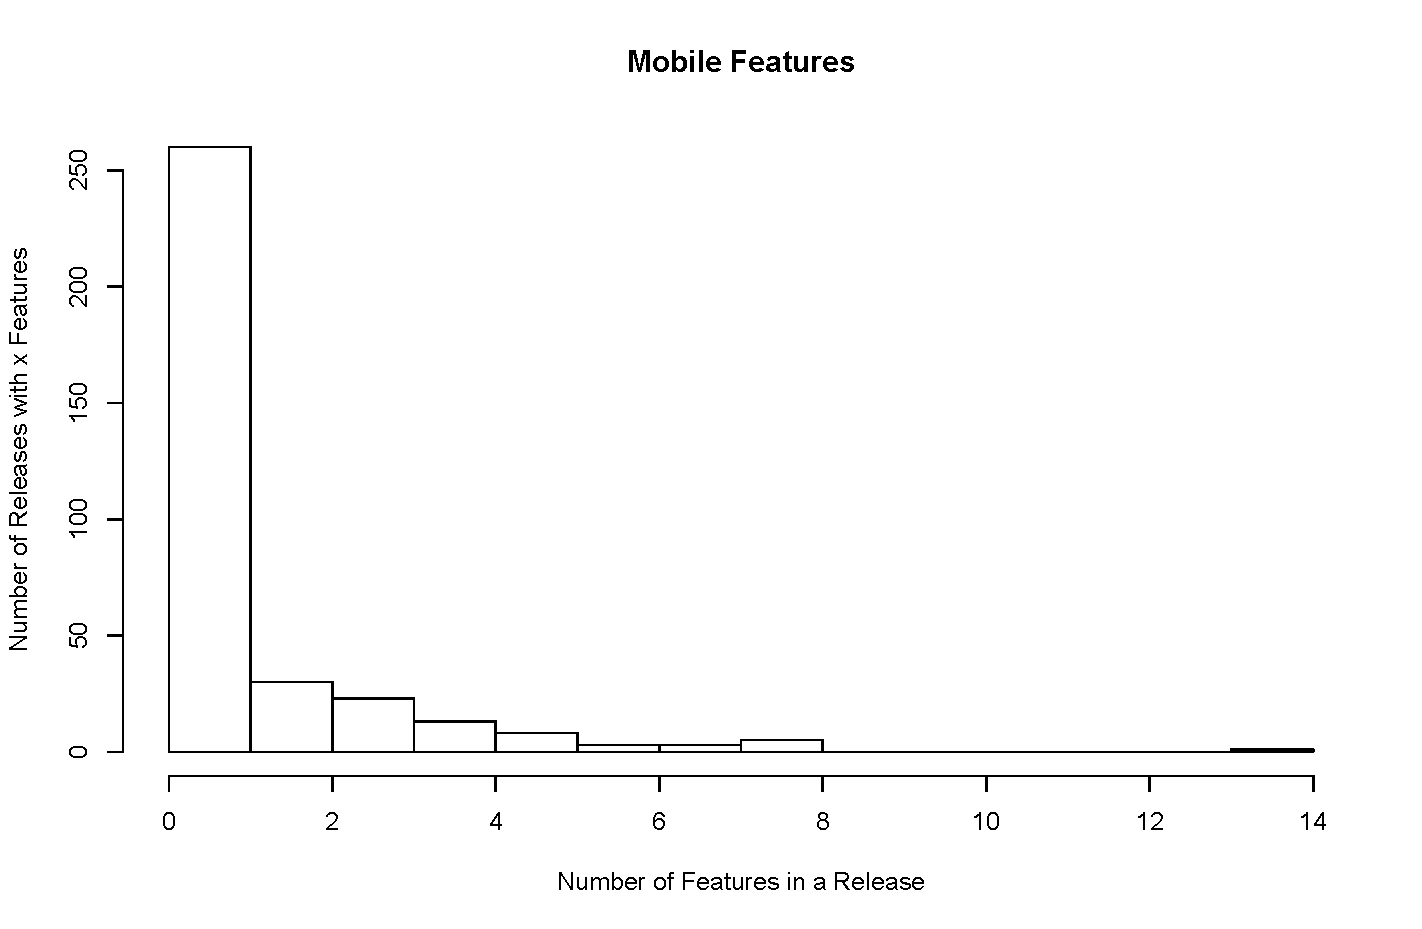
\includegraphics[width=.5\textwidth]{mobileFeaturesHist.pdf}
\label{fig:mobHist}
\caption{Mobile Features: this is a histogram of the frequency of releases containing a certain number of statements classified as features}
\end{center}
\end{figure}


The data collected for all research questions fit into histograms similar to Figure~\ref{fig:mobHist}. 
Figure~\ref{fig:mobHist} shows that the data does not follow a normal distribution, therefore, throughout the analysis we use the Wilcoxon Rank-Sum test to determine whether application categories exhibit significantly different behavior.


\subsection{Release Cycles}
While performing the calculations of the release cycles, we noticed instances where there would be a negative number of days between some releases.
For example, some release cycle lengths Tableau are: \textellipsis 33, 34, -68, 34, 34, 36, 33, 24, 28, 39, 28, 23, 36, -56, 20 \textellipsis\space . 
Such patterns only occurred in desktop applications and relate to the simultaneous maintenance of multiple branches. 
In Tableau, the release cycles of lengths 33, 34 correspond to the 4.1.x branch, release lengths -68, 34, 34, 36, 33, 24, 28, 39, 28, 23, 36 correspond to the 5.0.x branch, and release lengths -56, 20 correspond to the 5.1.x branch.



Negative release cycles not possible and so we decided to handle simultaneously maintained branches by tracing negative release cycles backwards until we found the first positive length of the release cycle and then continued to calculate release cycle lengths down each branch. 
So the sequence \textellipsis 33, 34, -68, 34, 34, 36, 33, 24, 28, 39, 28, 23, 36, -56, 20 \textellipsis becomes \textellipsis 33, 34, \textbf{36}, 34, 34, 36, 33, 24, 28, 39, 28, 23, 36, \textbf{3}, 20 \textellipsis when simultaneously maintained branches are factored in.

We did not observe this behavior in mobile or \sibs. We suspect that this is due to the nature distribution platforms for mobile applications.
Where desktop applications often have all their release notes stored on a centralized website or wiki, mobile applications will either show the release notes for the current release if on the Google Play or the Microsoft App Store (though some developers append notes as opposed to replacing them each release) or up to the previous 25 releases if on the iTunes App Store. 
If the developers do not maintain separate release notes on their own websites it does not make sense to maintain multiple simultaneous release branches for one platform because the release notes can quickly be replaced and leave users confused if for example they have version 5.0, but the most recent release notes are shown to be 4.9.5.
Multiple branches may be maintained across mobile platforms, but this is not evident because the release notes are stored across two different platforms (e.g. iTunes App Store and Google Play).




\MyParagraph{Outliers} The authors looked at the outliers from each of the application categories to determine if there were any irregularities.
For mobile applications, the longest cycle length appeared in the application Sleep Cycle Alarm with a length 345 days. 
There was no indication as to the delay, neither the release notes nor the developers twitter did not provide any insights as to why the release cycle was so long.

The sibling application OmniGraffle contained the longest release cycle of all application categories at 825 days. 
However, OmniGraffle appears to be the victim of missing release notes.
The version number suddenly jumps from 3.2.4 to 4.1.2, it is very likely that the documentation either lapsed, was deleted, or misplaced during the 825 day period between releases.
As such, the authors removed this data point from the calculations because it does not accurately represent a single release cycle. 
The next longest cycle length at 442 days belongs to the application Covenant Eyes, which during that cycle completed a large scale architectural change.

The desktop application with the longest cycle length is NDepend, a static analysis tool, which had a cycle length of 606 days. 
According to the release notes, the two year release cycle spanned the jump from .NET 1.0 to .NET 2.0 assemblies.
During that time, no new Visual studio was released, so perhaps the developers did not feel the need to update NDepend.


\subsection{Release Cycle Contents}

To analyze the release cycle contents after classification, we added up the instances of each category (bug, feature, enhancement, non-functional, gratitude, and feedback/contact) to create a summary of the release.

After each release was summarized, we pulled the information from each summary and grouped by statement category for each application of that type into lists. 
For example, Desktop Application 1 has two releases containing 2 bugs and 2 features and 4 bugs and 0 features. After being grouped by type desktop applications will have a list of bugs containing 2 and 4 and a list of features containing 2 and 0.
From these lists we calculated the statistics for what type of contents constitute a common release.

\subsubsection{Linear Models }

In addition analyzing the number of occurrences of each category, we also tried to generate a linear model for each of the different categories of application.

The linear model follows the following form, where category would be replaced with desktop, mobile or sibling:

\begin{multline}
$$time_{category} = \beta_{0} + \beta_{1}Bugs_{category} + \beta_{2}Features_{category} + \\ \beta_{3} Enhancements_{category} + \beta_{4} NonFunctional_{category} + Error $$
\end{multline}

We hoped to use this model to predict the length of a release cycle based on the contents of its release notes.

\section{Conclusions}


\subsection{\RQOne }



\begin{figure}
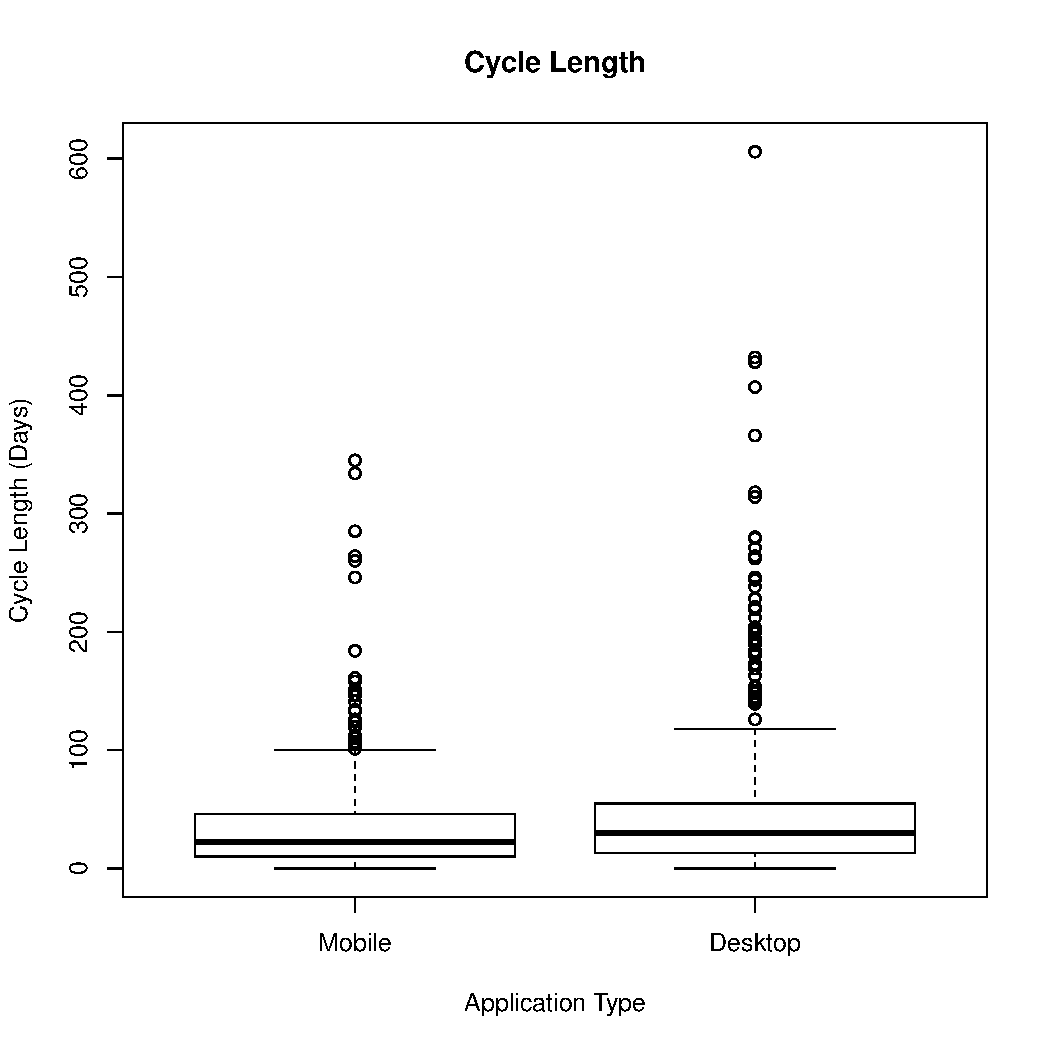
\includegraphics[width=.5\textwidth]{ShortCycleBoxPlot.pdf}
\label{fig:ShortCycleBox}
\caption{This box plot summarizes the information shown in Table~\ref{tab:sumshortcycles}}
\end{figure}

% latex table generated in R 3.1.2 by xtable 1.7-4 package
% Fri Dec 12 10:07:20 2014
\begin{table}[ht]
\centering
\caption{Cycle Summary} 
\begin{tabular}{rrrrr}
  & mean & median & std & max \\ 
 Mobile Applications & 35.784 & 22.500 & 43.591 & 345.000 \\ 
   \hline
Desktop Applications & 51.473 & 30.000 & 69.928 & 606.000 \\ 
  \end{tabular}
\end{table}




% latex table generated in R 3.1.2 by xtable 1.7-4 package
% Fri Dec 12 10:08:14 2014
\begin{table}[ht]
\centering
\caption{Cycle Length} 
\begin{tabular}{lr}
  \hline
Application Comparison & p-value \\ 
  \hline
Mobile vs Desktop & 6.35E-04 \\ 
   \hline
\end{tabular}
\end{table}




Research question one allows the authors to establish a baseline for the behavior of both only mobile applications and only desktop applications.
The authors originally suspected that mobile applications have shorter release cycles than desktop applications.
The data shows that this assumption is correct. 

As shown in Table~\ref{tab:sumshortcycles}, we found that both the mean and median for desktop applications' cycle lengths was larger than than of mobile applications. 
We believe that the median more accurately represents the characteristic cycle length because the cycle lengths do not exhibit a normal distribution as mentioned in Section~\ref{sec:analysis}. 

Given the difference in the maximum cycle lengths between the two categories of application, we expected a more substantial difference between the median cycle lengths.
However, the data indicates that the difference between the two is only about a week.
Table~\ref{tab:shortcycles} shows that mobile and desktop applications demonstrate statistically different behavior (p-value < 0.05).

We believe that the mobile applications have shorter release cycles because they were more likely developed in an agile paradigm than the desktop applications. 
The oldest mobile application was first released in 2009, 8 years after the agile manifesto was published. 
The oldest desktop application was first published in 2004, only 3 years after the agile manifesto was published so agile programming may not have had enough time to become a common practice during the early development of the desktop applications.
Additionally, during the initial development of some of the desktop applications, software was still distributed on disks or at least not as conveniently for users as automatic updates. 
The original need to physically update software may have created a culture of lengthened desktop release cycles.



\textit{In summary, mobile applications have distinctly shorter release cycles than desktop applications by 7.5 days.}


\subsection{\RQTwo }
Our second research question looks at whether the release cycles of \sibs tend to exhibit behavior closer to desktop or mobile behavior because research question one showed that mobile and desktop release cycles displayed different behavior.

Table~\ref{tab:sumcycles} adds another row to Table~\ref{tab:shortcycles} for sibling applications. 
Table~\ref{tab:sumcycles} shows that the mean and the maximum cycle length for the sibling applications lies between the mean and the maximum for desktop and mobile applications. 
Surprisingly, the median cycle length is lower than the mobile median cycle length. 
Additionally, there is no statistically significant difference between mobile and sibling applications, therefore we claim sibling applications release cycle lengths behave like mobile applications.


Sibling applications behaving like mobile applications is unexpected because almost all of the sibling applications were originally desktop applications that later had a sibling mobile application developed.
The two exceptions for this include Spotify, whose mobile application was released first, and SplashID, whose sibling applications were released on the same day.
Sibling desktop applications also made up a larger portion of the data points for this category (250 desktop points vs. 62 mobile points), so we anticipated sibling applications to behave more similarly to desktop applications.

The oldest sibling application is OmniGraffle, which first released in 2005.
However, unlike the desktop application category, OmniGraffle's age is an oddity among the sibling applications, with the next oldest being released 4 year later in 2009. 
This shows the potential hypothesis that age and release cycle length strongly correlated for future work.

\textit{In short, sibling applications exhibit release cycle lengths of mobile applications.}

\begin{figure}
\begin{center}
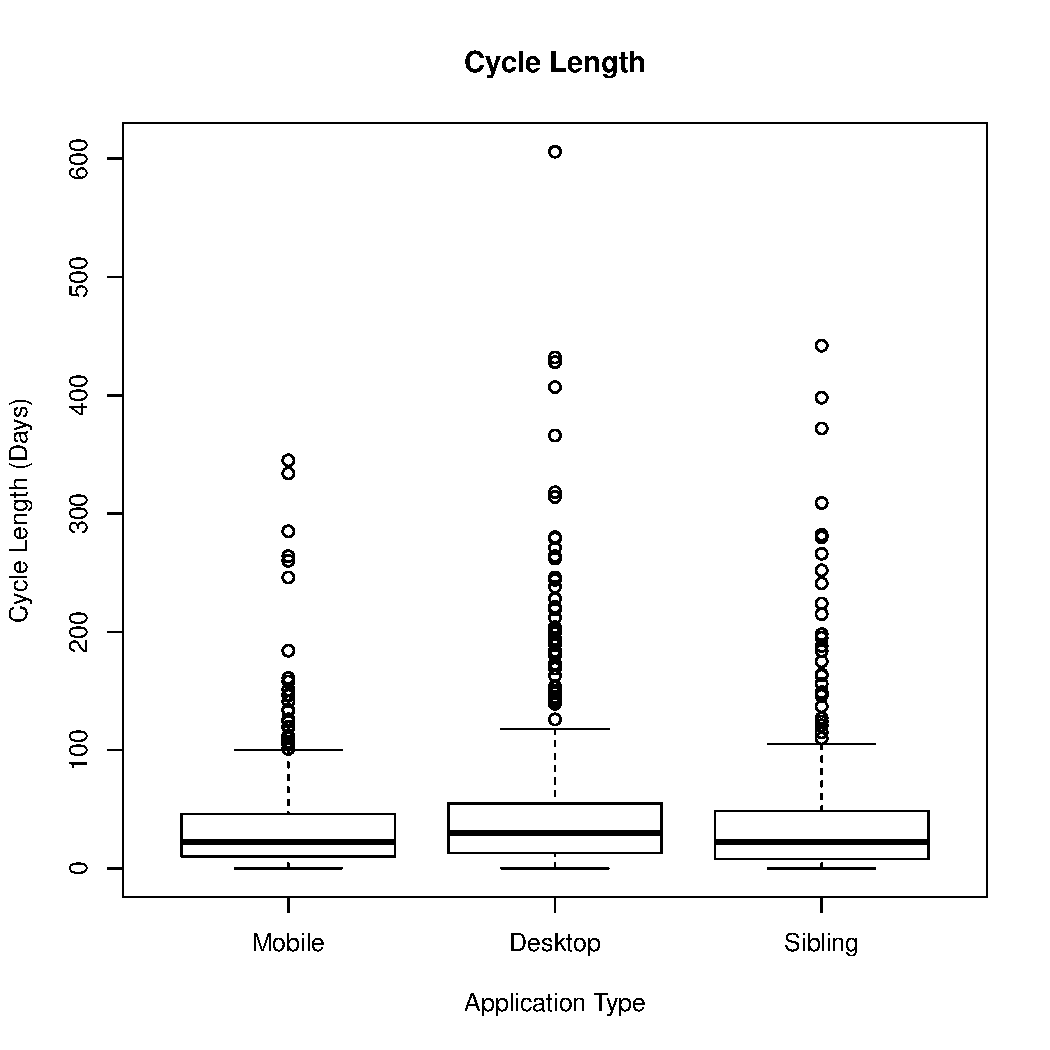
\includegraphics[width=.5\textwidth]{CycleBoxPlot.pdf}
\label{fig:CycleBox}
\caption{This box plot summarizes the information in Table~\ref{tab:sumcycles}}
\end{center}
\end{figure}

\begin{center}
% latex table generated in R 3.1.2 by xtable 1.7-4 package
% Fri Dec 12 10:07:20 2014
\begin{table}[ht]
\centering
\caption{Cycle Summary} 
\begin{tabular}{rrrr}
 mean & median & std & max \\ 
 35.784 & 22.500 & 43.591 & 345.000 \\ 
   \hline
51.473 & 30.000 & 69.928 & 606.000 \\ 
  43.283 & 22.000 & 64.215 & 442.000 \\ 
  \end{tabular}
\end{table}


\end{center}

\begin{center}
% latex table generated in R 3.1.2 by xtable 1.7-4 package
% Fri Dec 12 10:08:14 2014
\begin{table}[ht]
\centering
\caption{Cycle Length} 
\begin{tabular}{lr}
  \hline
Application Comparison & p-value \\ 
  \hline
Mobile vs Desktop & 7.54E-03 \\ 
  Mobile vs Sibling & 4.88E-01 \\ 
  Sibling vs Desktop & 2.18E-03 \\ 
   \hline
\end{tabular}
\label{tab:cycles}
\end{table}


\end{center}


\subsection{\RQThree }



\subsubsection{Bugs}

\begin{center}
% latex table generated in R 3.1.2 by xtable 1.7-4 package
% Fri Dec 12 15:19:53 2014
\begin{table}[ht]
\centering
\caption{Bug Summary} 
\begin{tabular}{rrrr}
 mean & median & std & max \\ 
 0.899 & 1.000 & 1.043 & 8.000 \\ 
   \hline
4.467 & 3.000 & 5.179 & 33.000 \\ 
  1.464 & 1.000 & 1.590 & 11.000 \\ 
  \end{tabular}
  \label{tab:sumBugs}
\end{table}


\end{center}

\begin{center}
% latex table generated in R 3.1.2 by xtable 1.7-4 package
% Fri Dec 12 10:08:14 2014
\begin{table}[ht]
\centering
\caption{Bugs} 
\begin{tabular}{lr}
  \hline
Application Comparison & p-value \\ 
  \hline
Mobile vs Desktop & 1.38E-16 \\ 
  Mobile vs Sibling & 1.14E-02 \\ 
  Sibling vs Desktop & 1.92E-10 \\ 
   \hline
\end{tabular}
\end{table}


\end{center}

Table~\ref{tab:sumBugs} contains a summary of the number of bugs found per release of each of the application categories. 
We once again use the median as our standard for comparison, which shows that desktop applications have more bugs per release than mobile or sibling applications. 

After looking at the causes for the maximum number of bugs being three times that the sibling application maximum number of bugs, we found that desktop applications were more likely to include release notes from publicly release beta builds. 
We searched each of the application categories corpus to look at instances of the word "beta."
We noticed that mobile applications mention beta features or accounts or mentions for supporting beta operating systems, but no versions are mentioned as being in beta. 
Likewise the only mentions of a beta version in the desktop sibling application.
Many of the desktop applications mention certain versions as being in beta.

The lack of public betas could be attributed to the mobile applications public distribution that automatically checks for updates applications to prevent customers from unknowingly downloading beta applications. 
It may be the result of the rating system; developers may fear releasing unstable versions that could permanently damage their ratings and thus their profits. 
The lack of beta versions in mobile applications could be a part of a future work.

Another reason desktop applications have more bugs per release than other categories may be that longer release cycles allow developers to spend more time testing and fixing bugs. 

Another influence on the disparity number of enhancements will discussed in the Threats to Validity.

\textit{Desktop applications exhibit more bugs per release than mobile or sibling applications}

\subsubsection{Features}

\begin{center}
% latex table generated in R 3.1.2 by xtable 1.7-4 package
% Fri Dec 12 15:19:53 2014
\begin{table}[ht]
\centering
\caption{Feature Summary} 
\begin{tabular}{rrrr}
 mean & median & std & max \\ 
 1.092 & 0.000 & 1.831 & 14.000 \\ 
   \hline
1.492 & 0.000 & 2.326 & 10.000 \\ 
  0.611 & 0.000 & 1.204 & 6.000 \\ 
  \end{tabular}
\end{table}


\end{center}

\begin{center}
% latex table generated in R 3.1.1 by xtable 1.7-4 package
% Thu Dec 11 20:41:40 2014
\begin{table}[ht]
\centering
\caption{Features} 
\begin{tabular}{lr}
  \hline
Application Comparison & p-value \\ 
  \hline
Mobile vs Desktop & 2.34E-01 \\ 
  Mobile vs Sibling & 5.45E-02 \\ 
  Sibling vs Desktop & 3.16E-03 \\ 
   \hline
\end{tabular}
\label{tab:features}
\end{table}


\end{center}

Table~\ref{tab:sumfeatures} contains a summary of the number of features found per release of each of the application categories. 
We were surprised to discover that the median value for the number of features for all categories was 0, but that the maximum values were relatively high.
We also noticed that mobile and desktop applications were essentially the same, while sibling applications followed a different behavior as shown in Table~\ref{tab:features}.

We believe that the low median and the high number of maximum features in a release can be attributed to an ebb and flow of development and maintenance. 
When looking at an overview of the occurrences of features the non zero numbers cluster together for a few releases and then are separated my many releases with no new features.

For the mobile applications, the maximum number of features was included in the release notes for the longest mobile cycle showing that for the full year the development team had added quite a few new things. 
For the desktop applications, maximum number of features in a release appeared Kaleidoscope after a relatively long release cycle of about half a year.

We believe one cause of the sparse number of features could be that developing sibling application bogs down developers as they try to translate ideas across two very different platforms. 

\textit{Sibling applications contain less features per release than desktop or mobile applications}
\subsubsection{Enhancements}

\begin{center}
% latex table generated in R 3.1.2 by xtable 1.7-4 package
% Fri Dec 12 15:19:53 2014
\begin{table}[ht]
\centering
\caption{Enhancement Summary} 
\begin{tabular}{rrrr}
 mean & median & std & max \\ 
 1.520 & 1.000 & 1.895 & 16.000 \\ 
   \hline
4.542 & 3.500 & 5.072 & 28.000 \\ 
  1.590 & 1.000 & 2.090 & 12.000 \\ 
  \end{tabular}
\end{table}


\end{center}

\begin{center}
% latex table generated in R 3.1.1 by xtable 1.7-4 package
% Thu Dec 11 20:41:40 2014
\begin{table}[ht]
\centering
\caption{Enhancements} 
\begin{tabular}{lr}
  \hline
Application Comparison & p-value \\ 
  \hline
Mobile vs Desktop & 5.49E-08 \\ 
  Mobile vs Sibling & 3.70E-01 \\ 
  Sibling vs Desktop & 2.01E-06 \\ 
   \hline
\end{tabular}
\end{table}


\end{center}

Table~\ref{tab:sumfeatures} contains a summary of the number of enhancements res found per release of each of the application categories. 
Similarly to the bugs per release, desktop applications exhibited more enhancements per release than mobile or sibling applications.
For the number of enhancements, mobile and sibling applications showed the same behavior as seen in Table~\ref{tab:enhancements}.

The largest amount of enhancements per desktop application appeared in Versions after a release cycle of 194 days.
Desktop applications in general may have more enhancements per release because longer release cycles give the developers more time to test their applications.
Desktop applications may also be better hiding their bugs as sometimes enhancements are used by developers to hide that bugs were present before.
The authors could not know the motivation behind each enhancement, bugs may be hidden beneath some of the enhancements for all application categories.

Another influence on the disparity number of enhancements will discussed in the Threats to Validity.


\textit{Desktop applications exhibit more enhancements per release than mobile or sibling applications}
\subsection{Linear Modeling of Behavior}




\begin{center}

\begin{table}
\begin{center}
\begin{tabular}{l c }
\hline
               & Mobile Applications \\
\hline
(Intercept)    & $23.77^{***}$ \\
               & $(3.46)$      \\
Bugs           & $1.52$        \\
               & $(2.57)$      \\
Features       & $6.95^{***}$  \\
               & $(1.43)$      \\
Enhancements   & $3.61^{*}$    \\
               & $(1.52)$      \\
Non-Functional & $2.06$        \\
               & $(3.58)$      \\
\hline
R$^2$          & 0.13          \\
Adj. R$^2$     & 0.12          \\
Num. obs.      & 346           \\
\hline
\multicolumn{2}{l}{\scriptsize{$^{***}p<0.001$, $^{**}p<0.01$, $^*p<0.05$}}
\end{tabular}
\caption{Statistical models}
\label{table:coefficients}
\end{center}
\end{table}


\end{center}


\begin{center}

\begin{table}
\begin{center}
\begin{tabular}{l c }
\hline
               & Desktop Applications \\
\hline
(Intercept)    & $45.12^{***}$ \\
               & $(10.20)$     \\
Bugs           & $-1.35$       \\
               & $(1.51)$      \\
Features       & $9.01^{*}$    \\
               & $(4.44)$      \\
Enhancements   & $2.45$        \\
               & $(2.11)$      \\
Non-Functional & $-8.78$       \\
               & $(7.47)$      \\
\hline
R$^2$          & 0.11          \\
Adj. R$^2$     & 0.08          \\
Num. obs.      & 120           \\
\hline
\multicolumn{2}{l}{\scriptsize{$^{***}p<0.001$, $^{**}p<0.01$, $^*p<0.05$}}
\end{tabular}
\caption{Statistical models}
\label{table:coefficients}
\end{center}
\end{table}


\end{center}

\begin{center}

\begin{table}
\begin{center}
\begin{tabular}{l c }
\hline
               & Sibling Applications \\
\hline
(Intercept)    & $30.38^{***}$ \\
               & $(5.15)$      \\
Bugs           & $-2.17$       \\
               & $(2.16)$      \\
Features       & $1.74$        \\
               & $(3.00)$      \\
Enhancements   & $6.61^{***}$  \\
               & $(1.80)$      \\
Non-Functional & $-3.42$       \\
               & $(2.60)$      \\
\hline
R$^2$          & 0.07          \\
Adj. R$^2$     & 0.06          \\
Num. obs.      & 239           \\
\hline
\multicolumn{2}{l}{\scriptsize{$^{***}p<0.001$, $^{**}p<0.01$, $^*p<0.05$}}
\end{tabular}
\caption{Statistical models}
\label{tab:sibModel}
\end{center}
\end{table}


\end{center}

Unfortunately, the correlation for our linear models was fairly awful however, we still believe some information may be drawn from our results.
One of the reasons we believe correlation to be so low is that these applications are likely on a release schedule.
Instead of using these models to predict the cycle length, we look at what types of release contents adds more time to a release.
We think that significant co-efficients with large values may indicate the type of release contents that are most likely to cause a delayed release. 

For mobile applications, both the number of features and enhancements significantly affect the length of the release.
The number of features has almost twice the influence on release cycle length as the enhancements. 

For desktop applications,  only the number of features in a release significantly affects cycle length, though the number of features will influence the release cycle length more strongly than the features in a mobile application.

For sibling applications, only the number of enhancements in a release affects the release cycle length.

Though these models are still in an infant stage, we believe they show promise for predicting what causes delays in releases.
Interestingly enough, none of the models demonstrated that the number of bug fixes in a release had an effect on the cycle length.
We believe this shows developers are willing to delay their releases for features and enhancements, but will choose to fix bugs in later releases rather than break schedule.


\subsubsection{Threats to Validity}

One of the most significant is business pressure to create applications that people want to buy.
Developers, marketing, or public relations, whoever is writing the release notes, write, whether intentionally or not, vaguely about the number of bugs or enhancements they address in each release. 
We considered every instance of "bug fixes" or "improvements" as a single statement, but in reality we do not know the exact number of bug fixes or enhancements per release unless they were specifically named.
One of the reasons we believe the mobile and sibling application bugs and enhancements to be so much lower than desktop applications is the introduction of vagueness.
Mobile application release platform require developers to include some release notes, which also contributes to the instances of vague releases because developers will include a placeholder "bug fixes and improvements" as a permanent release note.

Another threat to the validity of RQ3 is that there is a significant business pressure to create \sibs or move to mobile platforms on the market, there must be a reason that desktop applications were unable to migrate to mobile platforms. 
If the reason has to do with computational power, function, or code size, then it stands to reason that more complicated applications may have more bugs, making our comparison unbalanced.


\subsection{Gratitude and Feedback/Contact}

\begin{table*}[width=.5\textwidth]
\begin{tabular}{c c c c}
 & Desktop Applications & Mobile Applications & Sibling applications \\
Occurrences of Gratitude & 4 & 23 & 12 \\
Occurrences of Feedback/Contact & 3 & 40 & 21 \\
\end{tabular}
\label{tab:gratandfeed}
\caption{This table shows the occurrences of the gratitude and feedback/contact categories in each type of application}
\end{table*}

Though there were not an abundance of occurrences, there were still more mobile and sibling applications that expressed gratitude or mentioned user feedback, as shown in Table~\ref{tab:gratandfeed}.
From our findings about mobile applications and their lack of beta releases, the increased calls for feedback may be attributed to needing user feedback that does not come with a permanent rating.
Additionally, mobile applications display their release notes in a more public place so developers may want to show their gratitude toward users in an attempt to elicit better ratings or to entice them to buy the application.

\section{Implications}

\MyParagraph{For application developers:} application developers can use the preliminary information from our linear models to keep an eye on how many features and enhancements they plan to complete per application. For example in SCRUM development, developers chose tasks to complete within a certain period of time.
If developers are aware that features and enhancement are more likely to lengthen release cycles, then they can balance the number of those chosen with bug fixes so as not to overburden themselves.

\MyParagraph{For team management:} Our results show a significant skew in bugs in desktop applications. Therefore, managers may want to add extra members to the QA team or allow extra time for QA before releasing a desktop application. 
Looking at the results from our linear model, a manager may want to break up mobile and desktop applications with many features into several releases so the release dates are less likely to be delayed or simply schedule extra time for cycles with more releases.

\MyParagraph{For tool builders:} The data generated by our research may show a higher concentration of bugs in each desktop application release. 
A tool builder may want to look through our data of all bugs to see what bugs plague desktop developers most often and try to help them avoid that.
Also, our research showed that sibling applications have a low number of features added per release.
If a tool builder wanted to help sibling application developers find and easier way to transition ideas across the platforms, then developers may be able to spend more time developing new features for sibling applications.

\MyParagraph{For researchers:} Researchers may find our results useful when doing research on mobile applications.
Also, for future work we may be able to generate a keywords dictionary or bigram dictionary based on our classification of statements that will allow them to perform more data mining on release notes.
This would be similar to what Yu \cite{YuChangeLogs} attempted, but with keywords drawn from concrete examples.


\section{Related Work}

Gall et al. \cite{GallSoftwareEv} developed a product release database for telecommunication switching system that automatically generated release notes based on the source code.
Like Gall et al., we plan to analyze software using the release histories provided by developers to derive information about software. 
However, instead of focusing on a single application, we will use information to compare applications on different platforms. 
In addition, the release notes we analyze are not generated based on the source code, but are disclosed by the developer.

Tsay et al. \cite{TsayOpenSourceMining} paper presents experiences, including the tools, techniques and pitfalls, in mining open source release histories, and specifically shows that many factors make automating the retrieval of release history information difficult, such as the many sources of data, a lack of relevant standards and a disparity of tools used to create releases. These are the similar problems we've found in our research.
The different thing from our recent research is that the projects quantity in this paper is very small, but number of versions of each project is very big. For example they collected 1579 distinct releases from 22 different open source projects, so on average 72 release versions per project. However, we focus on more types of software but less release version.

Yu \cite{YuChangeLogs} uses text data mining to extract information from change logs and release notes develop a mathematical model to represent software evolution based on predetermined keywords. Using the model, Yu traced the recurrences of issues across a single project.
Similarly our research mines release notes to gather information about the nature of software bugs and features, but ours attempts to use the data to compare different applications. 
Apart from version numbers and dates, our research steers away from filtering out information solely due to predefined keywords because positive spin, marketing terms, and buzz words interfere with simple collection of data. 
The inconsistencies in language across applications and companies is the reason we originally looked into naive Bayes classifiers to better assess the nature of statements in release notes.

Shobe et al. \cite{ShobeMapping} present an empirical study on the release naming and structure in three open source projects: Google Chrome, GNU gcc, and Subversion.  
The projected application requires forming a training set for a source-code change prediction model from the committed source code history are needed.
Our research also mines histories, but we focus less on developing a machine learning engine and more on potentially using one as a tool to help us perform classifications.

Wright and Perry \cite{WrightPitfalls} discusses early results from a set of multiple semi-structured interviews with practicing release engineers and focus on why release process faults and failures occur, how organizations recover from them, and how they can be predicted, avoided or prevented in the future.
Our research only seeks to look at the frequency, but Wright and Perry's interviews mentioned some root causes such as size, funding, and modularity that affect the frequency of release cycles.

Moreno et al. \cite{Laura} introduce ARENA (Automatic Release Notes generator), an approach for the automatic generation of release notes.
In the process of generating release notes, Laura et al. manually classified release notes to see what they consisted of like our paper. Fortunately many of the categories were similar, though Laura et al. identified many more categories depending on what was being modified or added.
However, this study was less concerned with comparing applications and more focused on generating release notes from code changes.

D. S. Cruzes \cite{Cruzes} paper provides guidance on how to properly conduct qualitative thematic coding. 
All of the statements we classified we according to the process laid out in Cruzes' paper to give our data validity. 
However, Cruzes' work does not specifically apply his method to a particular case to perform research as we have in this paper.



G. Antoniol  et al. \cite{Antoiol} investigate whether the test submitted for bug tracking systems is a bug or an enhancement. 
Like this study, software engineers manually classify text as either a bug or enhancement.
Antoniol et al.'s work was done with more engineers on a larger scale and also compared their manual results to automatically classified determined labels.
However, Antoniol et al.'s focus was the extension of use of the Mozilla bug tracking systems to track more than just bugs, while our was on comparing applications.


 K. Herzig et al. \cite{HerzigMis} looked at the misclassification of bug reports in open source projects. After manually examining issues they found that 40\% did not have any bugs. 
 Like our paper they also classified issues relating to bugs, features, and enhancements, but once again, their methods are focused on a system as opposed the applications in the system.
 Additionally, they looked at open source projects bug tracking systems which allow for tagging of issues as opposed to release notes.
 

 K. Herzig et al. \cite{HerzigData} look at the evolution of software projects using a large Mozilla open source project as their data source. They are able to populate a database with the release history as well include normally hidden information such as merge points.
 In this paper, Herzig et al. had access to the source code and version control system which allowed them finer grained analysis of the program. Our paper choses to use release notes with no code because we wanted to include proprietary projects in our analysis. We also look more at the characteristics of each release compared to the cycle length as opposed to monitoring changes made throughout the project's history.
 


% That's all folks!
\bibliographystyle{acm}
\bibliography{relatedwork}


\end{document}
